% Sketch output, version 0.3 (build 2d, Wed Apr 20 23:38:45 2011)
% Output language: PGF/TikZ,LaTeX
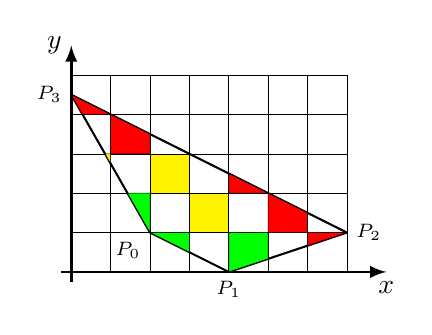
\begin{tikzpicture}[line join=round,line width=0.2pt,>=latex]
\filldraw[fill=none,line width=0.75pt](1,.5)--(2,0)--(3.5,.5)--(0,2.25)--cycle;
\draw(0,2.5)--(3.5,2.5);
\draw(0,2)--(3.5,2);
\draw(0,1.5)--(3.5,1.5);
\draw(0,1)--(3.5,1);
\draw(0,.5)--(3.5,.5);
\draw(0,0)--(3.5,0);
\draw(3.5,0)--(3.5,2.5);
\draw(3,0)--(3,2.5);
\draw(2.5,0)--(2.5,2.5);
\draw(2,0)--(2,2.5);
\draw(1.5,0)--(1.5,2.5);
\draw(1,0)--(1,2.5);
\draw(.5,0)--(.5,2.5);
\draw(0,0)--(0,2.5);
\filldraw[fill=red](3,.333)--(3.5,.5)--(3,.5)--cycle;
\filldraw[fill=red](2.5,.5)--(3,.5)--(3,.75)--(2.5,1)--cycle;
\filldraw[fill=red](2,1.25)--(2,1)--(2.5,1)--cycle;
\filldraw[fill=red](.5,2)--(.5,1.5)--(1,1.5)--(1,1.75)--cycle;
\filldraw[fill=red](0,2.25)--(.143,2)--(.5,2)--cycle;
\filldraw[fill=yellow](1.5,.5)--(2,.5)--(2,1)--(1.5,1)--cycle;
\filldraw[fill=yellow](1,1.5)--(1,1)--(1.5,1)--(1.5,1.5)--cycle;
\filldraw[fill=yellow](.5,1.5)--(.5,1.375)--(.429,1.5)--cycle;
\filldraw[fill=green](2,0)--(2.5,.167)--(2.5,.5)--(2,.5)--cycle;
\filldraw[fill=green](1,.5)--(1.5,.25)--(1.5,.5)--cycle;
\filldraw[fill=green](1,.5)--(1,1)--(.714,1)--cycle;
\draw[->,line width=1pt](0,-.125)--(0,2.875);
\draw[->,line width=1pt](-.125,0)--(4,0);

    \coordinate [label=below:$x$] (X) at (4,0);
    \coordinate [label=left:$y$] (Y) at (0,2.875);
  
    \coordinate [label=225:\scriptsize$P_0$] (p0) at (1,.5);
    \coordinate [label=270:\scriptsize$P_1$] (p1) at (2,0);
    \coordinate [label=000:\scriptsize$P_2$] (p2) at (3.5,.5);
    \coordinate [label=180:\scriptsize$P_3$] (p3) at (0,2.25);
  \end{tikzpicture}% End sketch output
